\chapter{Annotation Service}

To enable the pathologist to make annotations in the first place, a GUI needs to be offered by the service. This GUI will be developed in iterations with the help of a number of pathologists to adapt it to their wishes and grant the best possible usability. The basic concept of the first iteration will be based on the Microdraw\footnote{See \url{https://github.com/r03ert0/microdraw} for more information on the Microdraw project} GUI (see fig. 2.5).

\begin{figure}[H]
	\begin{center}
		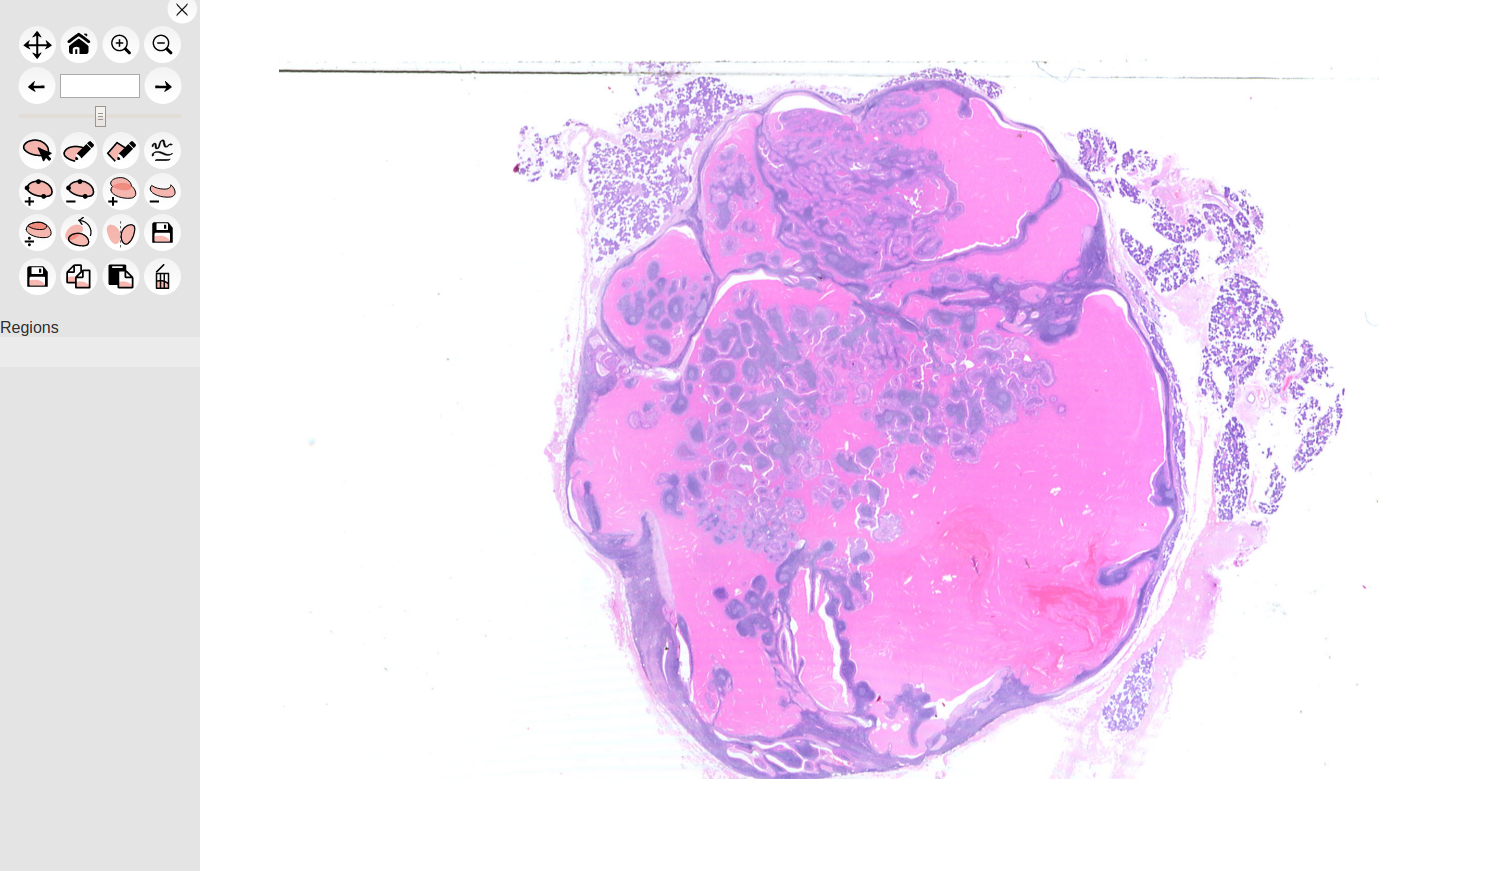
\includegraphics[scale=0.2]{img/microdrawUI.png}
		\caption{Microdraw GUI with opened WSI}
		\label{fig:fig2.5}
	\end{center}
\end{figure}

Microdraw is a webbased annotation tool, which describes itself as

\begin{quotation}
	"[...] a collaborative vectorial annotation tool for ultra high resolution data, such as that produced by high-throughput histology." \cite{web:microdraw}
\end{quotation}

Therefore, the GUI of the Annotation Service, or Annotation Service Viewer (ASV)\nmc{ASV}{Annotation Service Viewer}, will run as a web application in a browser. Annotations will be made by selecting a shape or annotation method from the various tools in the toolbar (see the gray bar on the left in fig. 2.5). After selecting the area to be annotated, an actual description of that area can be made via keyboard input.

When the pathologist is done or wants to save the made annotations, the Annotation Service will create a file in which they will be persisted in. Only one WSI can be opened in one ASV at a time.

\section{Methodology}
% how are WSIs usually viewed and annotated?
% iterative approach with UX evaluation by pathologist
\subsection{Parts of the Annotation Service}
% 2 basic units: server & client
% browser application for os independence
\subsubsection{Annotation Service Viewer}
% microdraw as base
\subsubsection{Annotation Service Server}
% web browser needs server to deliver images
	% local for now

\subsection{Functionality}
% shortcuts, funtions, etc. pp.

\section{Implementation}
% what was used for implementation
\subsection{Technologies and Frameworks}
% openslide, openslide web server
% python web server, flask, openslide, java script, html5, css
\subsection{Local Web Server}
% documentation
\subsection{Web Application}
% documentation